\section{Fine-tuning the model}

We have achieved decent performance of the model using only synthetic images during training. However, the performance could be improved since the synthetic data can't cover all the possible real case scenarios. In this section, we talk about using real images to fine-tune our model. We propose two approaches. The first idea is that we will merge real images with synthetic in the training dataset and train the model from scratch again. The second approach is to use real data to only fine-tune fully-connected layers responsible for the classification. 

\subsection{Data}

In Section \ref{sec:inputdata} we mentioned that the real data used in this work needed to be manually cut out using a 50x50 window with just one object present in the image. Cropped images were then divided into 3 datasets: training, validation and testing dataset. Each dataset contains 50 images per class, giving a total of 300 images per dataset. However, to train the network, this is a very small amount of data. 
To increase the size of the dataset we implement augmentation techniques mentioned in the Section \ref{sec:parametersNetwork} and depicted in the Figure \ref{fig:agcutline}. This gives us a total of 1800 images for the training dataset used to fine-tune the network. 

\begin{figure}[!h]
   \centering
    \begin{subfigure}[t]{.15\textwidth}
        \centering
        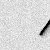
\includegraphics[width=\textwidth]{images/cutlineAg.png}
        \label{fig:cutlineag}
        \caption{}
    \end{subfigure}
    %\hfill
    \begin{subfigure}[t]{.15\textwidth}
        \centering
        
\includegraphics[width=\textwidth]{images/cutlineAg90.png}
        \label{fig:cutlineag90}
        \caption{}
    \end{subfigure}
    %\hfill
    \begin{subfigure}[t]{.15\textwidth}
        \centering
        
\includegraphics[width=\textwidth]{images/cutlineAg180.png}
        \label{fig:cutlineag180}
        \caption{}
    \end{subfigure}
    %\hfill
    \begin{subfigure}[t]{.15\textwidth}
        \centering
        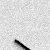
\includegraphics[width=\textwidth]{images/cutlineAg270.png}
        \label{fig:cutlineag270}
        \caption{}
    \end{subfigure}
    %\hfill
    \begin{subfigure}[t]{.15\textwidth}
        \centering
        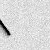
\includegraphics[width=\textwidth]{images/cutlineAgflipVodorovne.png}
        \label{fig:cutlineaghor}
        \caption{}
    \end{subfigure}
    %\hfill
    \begin{subfigure}[t]{.15\textwidth}
        \centering
        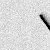
\includegraphics[width=\textwidth]{images/cutlineAgZvisle.png}
        \label{fig:cutlineagvert}
        \caption{}
    \end{subfigure}
    %\hfill
    \caption[Augmentation techniques applied to image of cut streak.]
    {Augmentation techniques applied to image of cut streak.(a) Original image, (b) Rotated by 90 °, (c) Rotated by 180 °, (d) Rotated by 270 °, (e) Flipped horizontally, (f) Flipped vertically. }
    \label{fig:agcutline}
\end{figure}

\subsection{Training on merged data} \label{subsec:mergedmodel} 

The first proposed approach is to merge synthetic training data with the real training data into one dataset and use it to train the model. Using this method we have gone through an extensive process of tuning the hyperparameters, similar to what we explained in Section \ref{sec:modelselection}. We have trained more than 50 models and settled on the best-performing one with the following parameters: 

\begin{itemize}
    \setlength\itemsep{1px}
    \item activation function Leaky RELU with a slope of 0.05
    \item batch size of 32
    \item optimizer ADAM with betas = 0.9, 0.999
    \item starting learning rate of $1e^{-3}$
    \item exponential scheduler with $\gamma$ = 0.9
    \item dropout in fully-connected layer with probability of 0.5
    \item L2 regularization with $\lambda$ set to $1e^{-5}$
\end{itemize}

The model was evaluated on the validation set and achieved an accuracy of 94.67 \% on the real data and 99.33 \% on the synthetic data. The training process of the model is depicted in the Figure \ref{fig:lossaccm11}. Comparing this to the final model in Section \ref{subsec:finalmodel} we have improved the performance on the validation set (with real data) significantly. 

\begin{figure}[!h]
\centering
    \begin{subfigure}[t]{.45\textwidth}
        \centering
        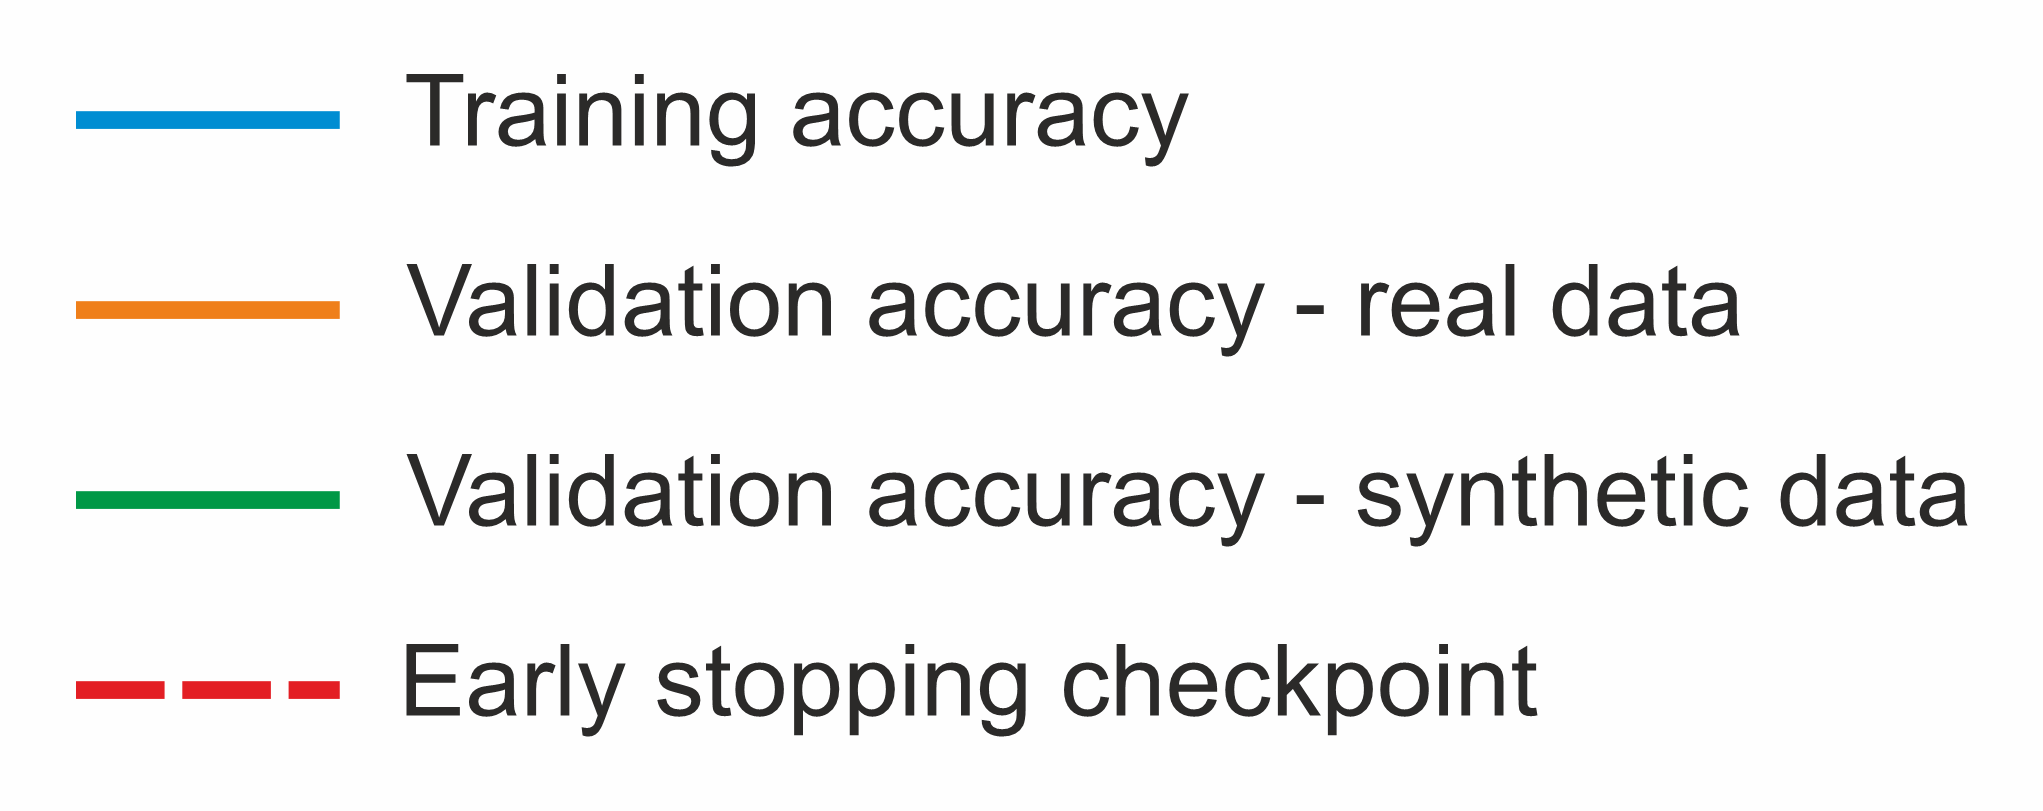
\includegraphics[width=.7\textwidth]{images/popisAc.png}
        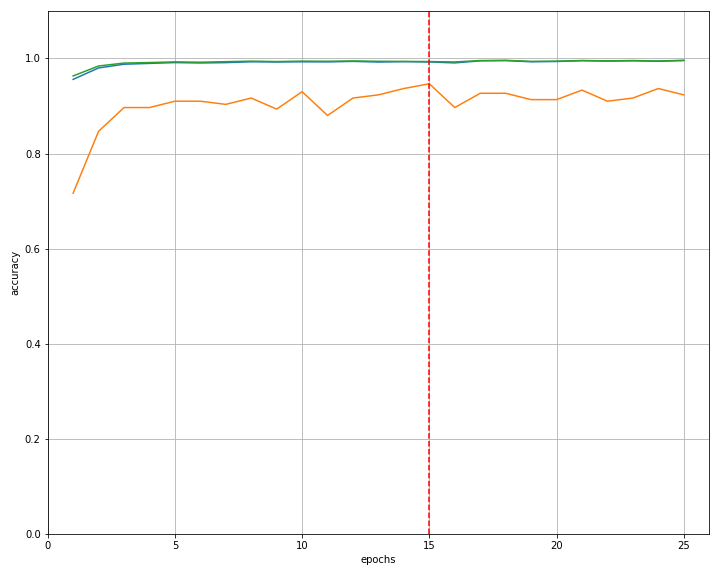
\includegraphics[width=\textwidth]{images/accuracy13r_0.png}
        \caption{The accuracy during training.}
        \label{fig:accm11}
    \end{subfigure}
    \begin{subfigure}[t]{.45\textwidth}
        \centering
        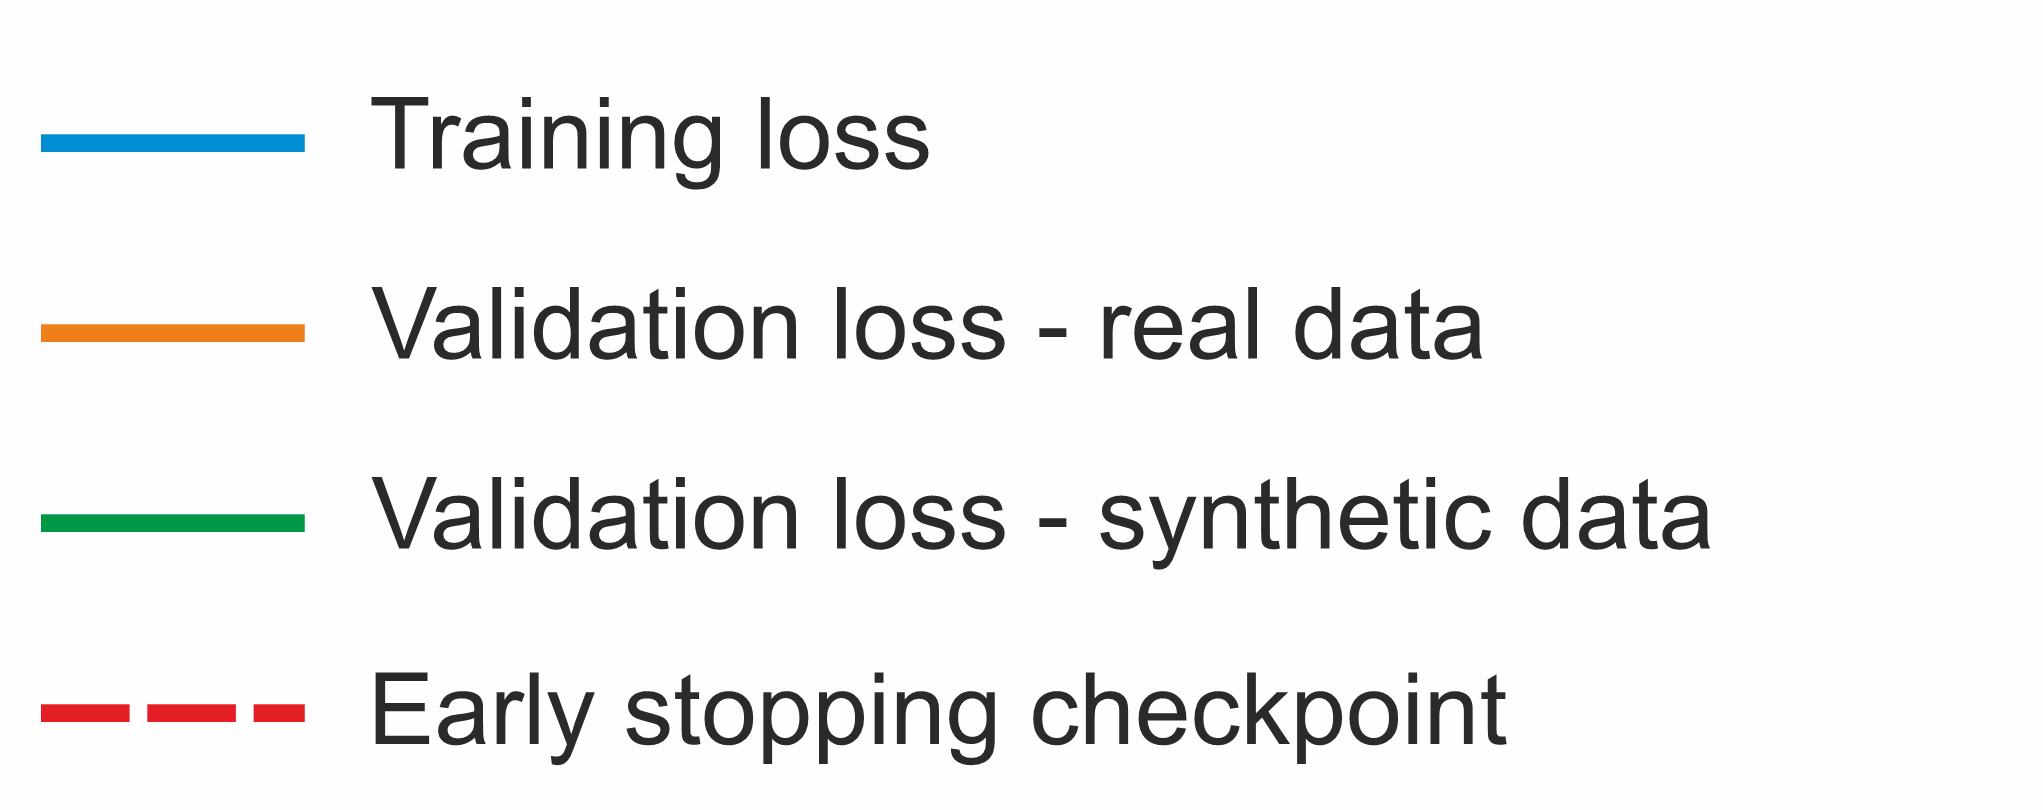
\includegraphics[width=.7\textwidth]{images/popisLoss.png}
        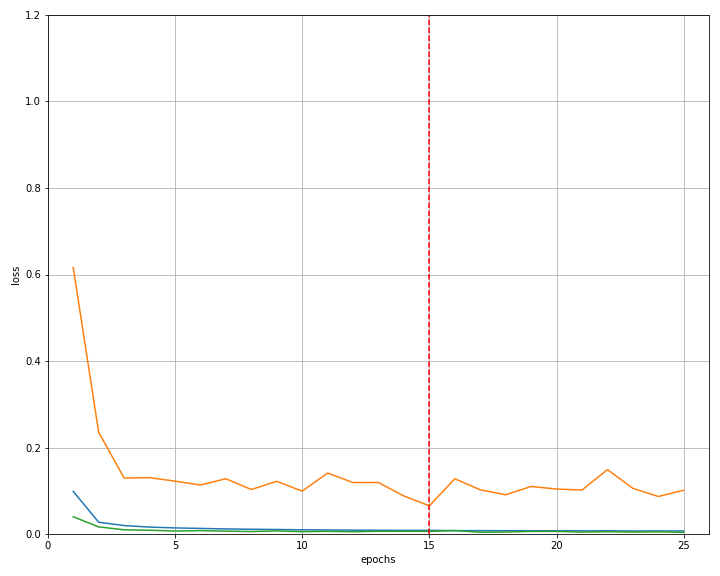
\includegraphics[width=\textwidth]{images/losses13r_0.png}
        \caption{The loss during training.}
        \label{fig:lossm11}
    \end{subfigure}

    \caption{The evolution of the loss and accuracy during training of the model with the merged dataset of real and synthetic images.}
    \label{fig:lossaccm11}
\end{figure}
\subsection{Fine-tuning fully-connected layers} \label{subsec:fcmodel}

The second approach is to fine-tune only the fully connected layers with the real data. The first convolutional/pooling layers that perform the feature extraction are frozen, which means that during training their weights are not updated. This way we are using a feature extractor trained on synthetic data and with real data we improve only the classification of the network. 

We are using the trained final model from Section \ref{subsec:finalmodel} as a feature extractor, which achieved the accuracy of 81.00 \% on the validation set of real data. Again we are testing various hyperparameters to improve our model. Based on the extensive training we have established a model with following parameters: 

\begin{itemize}
    \setlength\itemsep{1px}
    \item activation function Leaky RELU with a slope of 0.05
    \item batch size of 64
    \item optimizer ADAM with betas = 0.9, 0.999
    \item starting learning rate of $1e^{-3}$
    \item exponential scheduler with $\gamma$ = 0.9
    \item dropout in fully-connected layer with probability of 0.5
    \item L2 regularization with $\lambda$ set to $1e^{-5}$
\end{itemize}

The model achieved an accuracy of 94.33 \% on the real data and 87 \% on the synthetic data on the validation set. While the accuracy on the real data has improved from the model in Section \ref{subsec:finalmodel}, the performance on the synthetic data has decreased significantly. 
The evolution of loss and accuracy during training is illustrated in the Figure \ref{fig:lossaccm33}. 


\begin{figure}[!h]
\centering
    \begin{subfigure}[t]{.45\textwidth}
        \centering
        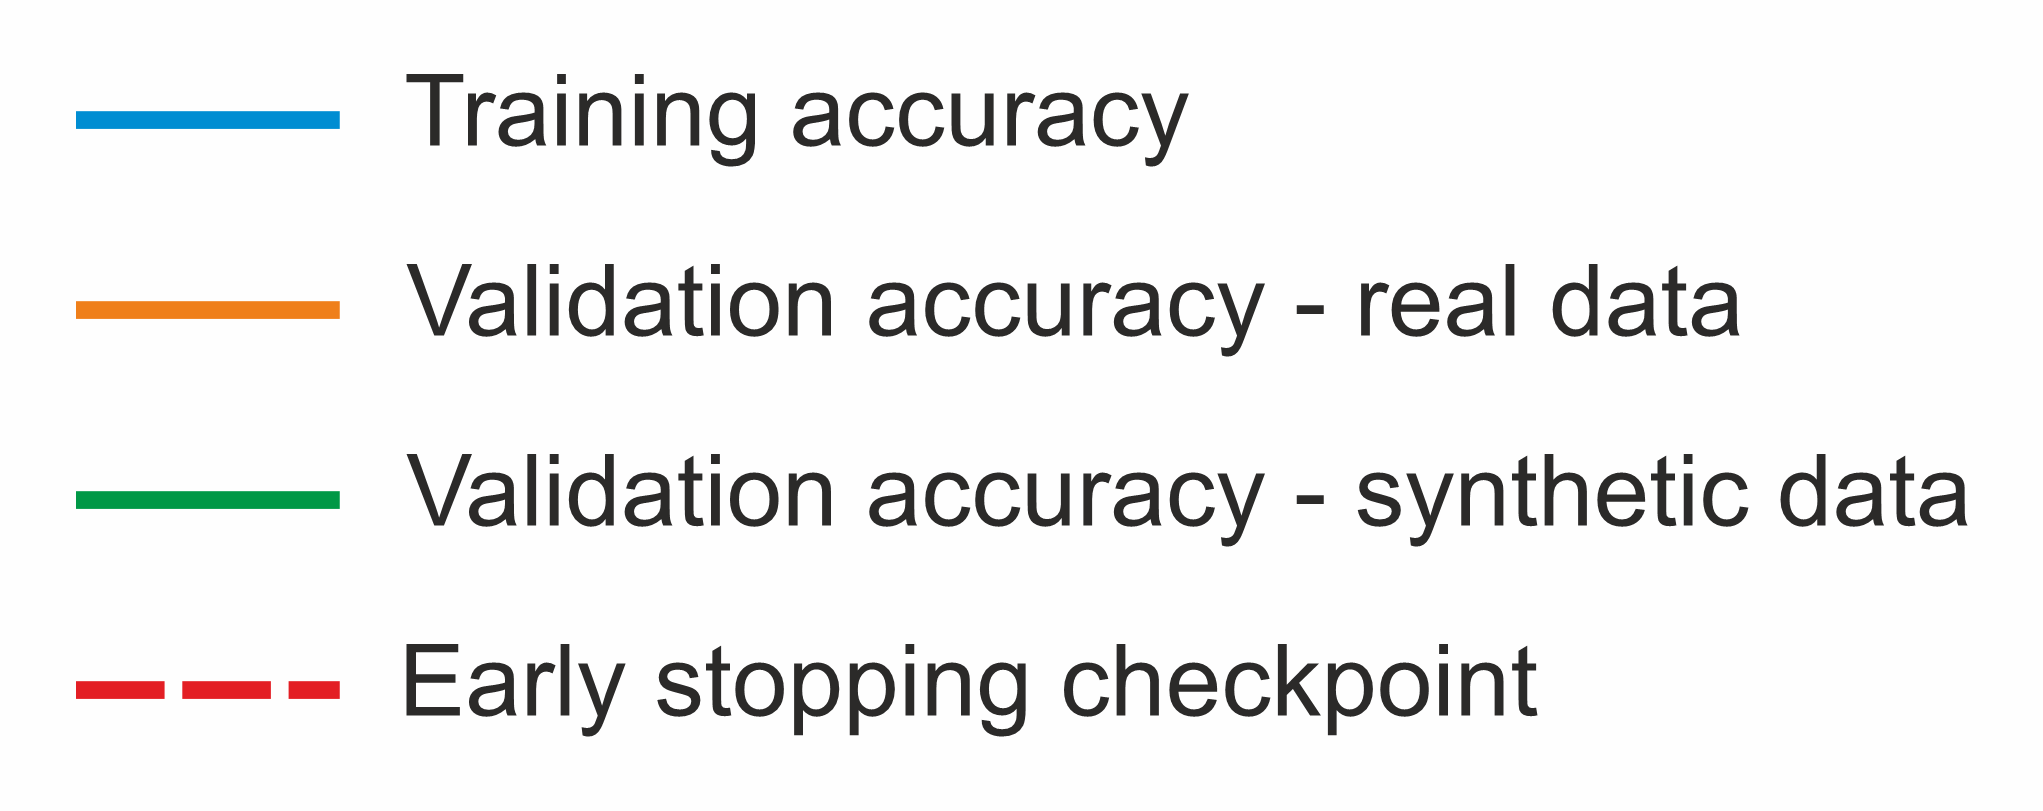
\includegraphics[width=.7\textwidth]{images/popisAc.png}
        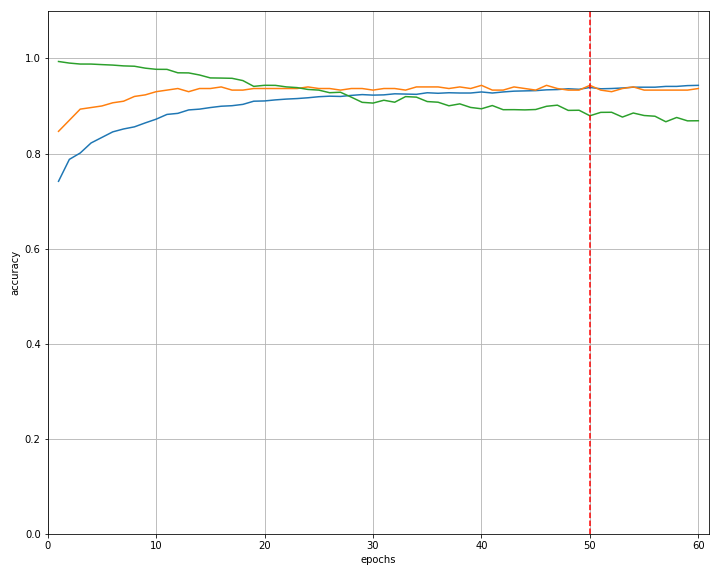
\includegraphics[width=\textwidth]{images/accuracy14fe_0.png}
        \caption{The accuracy during training.}
        \label{fig:accm33}
    \end{subfigure}
    \begin{subfigure}[t]{.45\textwidth}
        \centering
        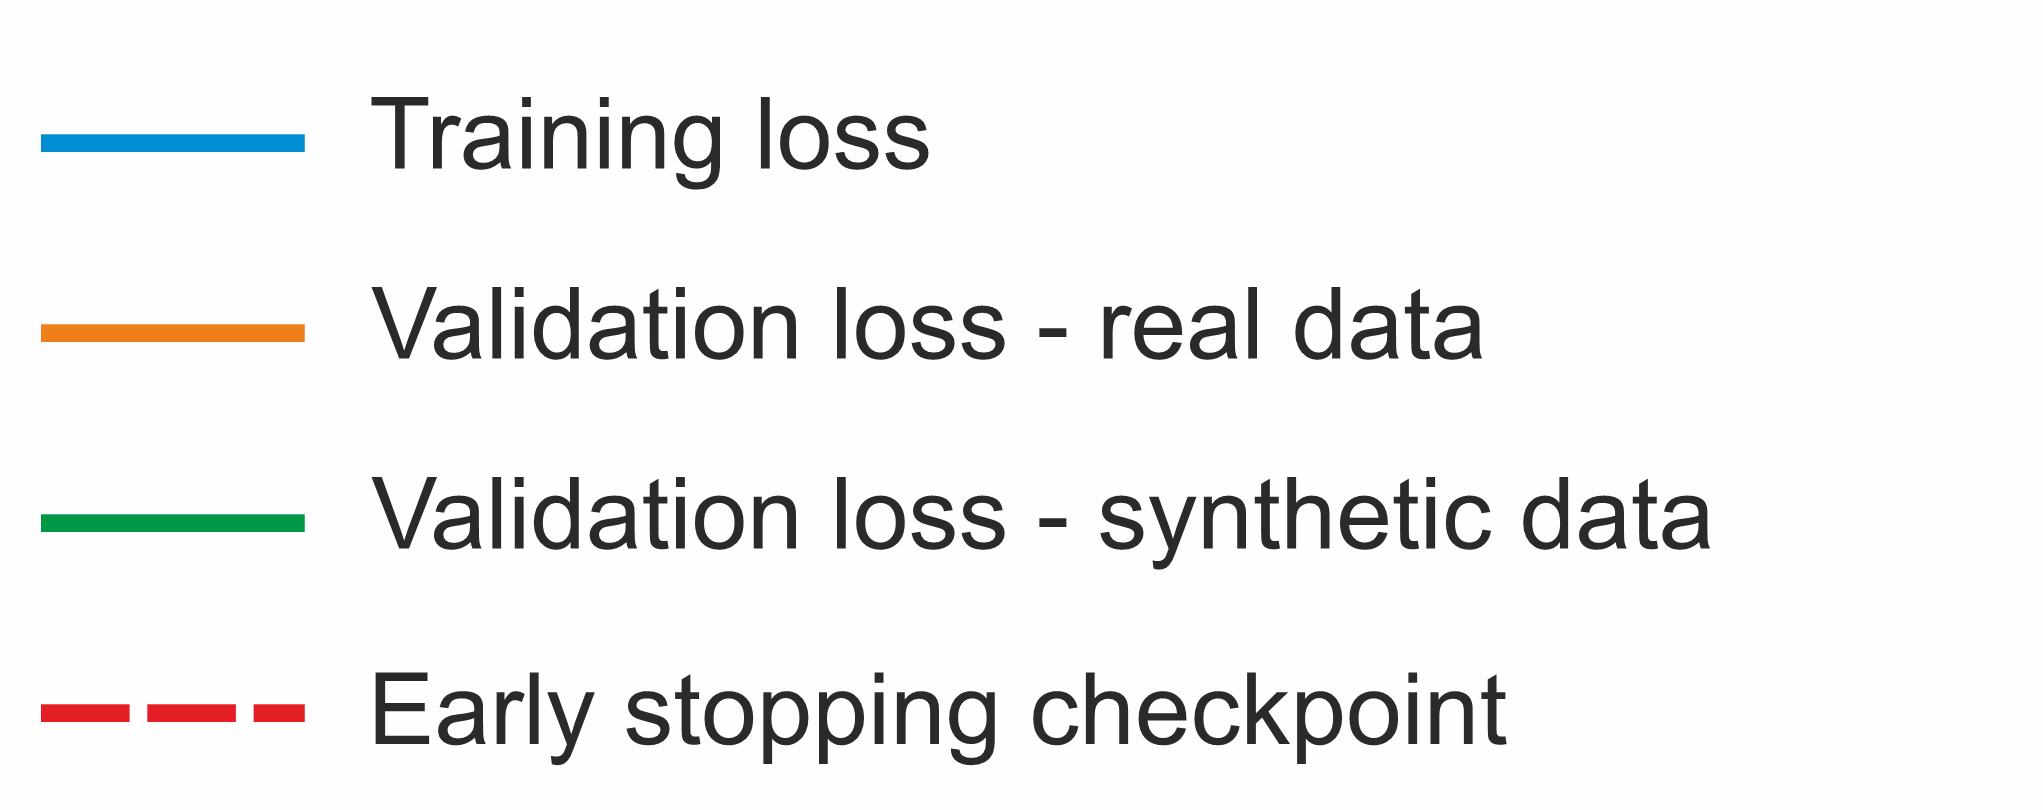
\includegraphics[width=.7\textwidth]{images/popisLoss.png}
        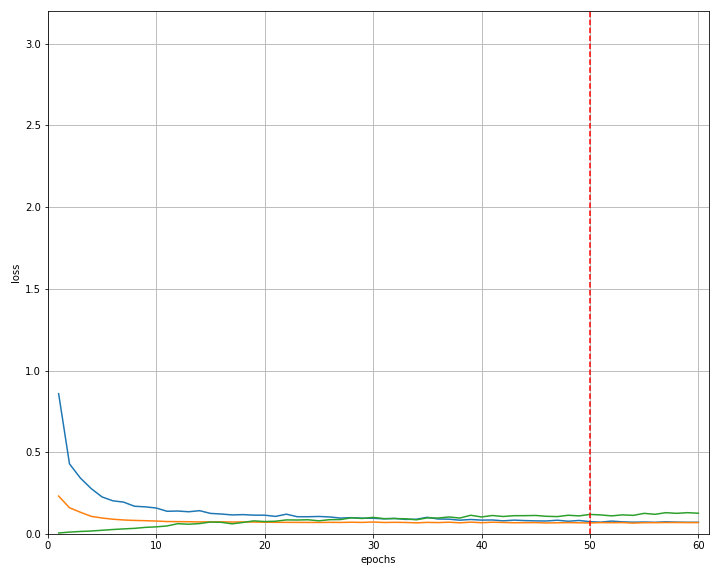
\includegraphics[width=\textwidth]{images/losses14fe_0.png}
        \caption{The loss during training.}
        \label{fig:lossm33}
    \end{subfigure}

    \caption{The evolution of the loss and accuracy during training of the model that has fine-tuned fully-connected layers with real data.}
    \label{fig:lossaccm33}
\end{figure}